\documentclass[14pt,a4paper]{scrartcl}
\usepackage{cmap}
\usepackage[utf8]{inputenc}
\usepackage[T1,T2A]{fontenc}
\usepackage[english,russian]{babel}
\usepackage{relsize}
\usepackage{graphicx}
\usepackage{subfigure}
\usepackage{mathtools}
\usepackage{amssymb}
\usepackage{float}
\usepackage{sidecap}
\usepackage{wrapfig}
\usepackage{caption}
\usepackage[table,xcdraw]{xcolor}
\usepackage{minted}
\usepackage{tcolorbox}
\usepackage{enumitem}
\makeatletter

\renewcommand{\thesubsection}{\arabic{subsection}}

\newenvironment{sqcases}{%
	\matrix@check\sqcases\env@sqcases
}{%
	\endarray\right.%
}
\def\env@sqcases{%
	\let\@ifnextchar\new@ifnextchar
	\left\lbrack
	\def\arraystretch{1.2}%
	\array{@{}l@{\quad}l@{}}%
}
\makeatother

\begin{document}
	\begin{titlepage}
		\begin{center}
			\large
			МИНИСТЕРСТВО ОБРАЗОВАНИЯ И НАУКИ\\ РОССИЙСКОЙ ФЕДЕРАЦИИ
			
			\vspace{0.5cm}
			
			МГТУ им Н.Э.Баумана
			\vspace{0.25cm}
			
			Факультет ФН
			
			Кафедра вычислительной математики и математической физики
			\vfill
			
			
			Соколов Арсений Андреевич\\
			\vfill
			
			
			{\LARGE Семинар от 16.05.20\\ по основам сеточных методов \\[2mm]
			}
			\bigskip
			
			3 курс, группа ФН11-63Б\\
			Вариант 3
		\end{center}
		\vfill
		
		\newlength{\ML}
		\settowidth{\ML}{«\underline{\hspace{0.7cm}}» \underline{\hspace{2cm}}}
		\hfill\begin{minipage}{0.4\textwidth}
			Преподаватель\\
			\underline{\hspace{3cm}} В.\,А.~Кутыркин\\
			«\underline{\hspace{0.7cm}}» \underline{\hspace{1.71cm}} 2020 г.
		\end{minipage}%
		\bigskip
		
		
		\vfill
		
		\begin{center}
			Москва, 2020 г.
		\end{center}
	\end{titlepage}
	Семинар от 17.05.2020, Основы сеточных методов , ФН11-63Б, вариант 3,
	Соколов Арсений Андреевич, Кутыркин Владимир Андреевич
	
	\section*{Задачи для решения на семинаре}
	
	\textbf{Задача 1.}\\ Для ограниченной односвязной области с гладкой границей нарисовать равномерную сетку, выделив на ней «заштрихованный» 1-приграничный слой $\Gamma_1 $ для сетки на этой области.
	
	\textbf{Решение.}
	
	Рассмотрим в качестве искомой области $\underline{G}$ круг $x^2 + y^2 < R^2$. Тогда гладкой границей $\gamma$ будет окружность $x^2 + y^2 = R^2$. Двумерная равномерная сетка примет вид:
	
	\begin{equation*}
		\underline{C} = \left\langle (x_k = kh, y_m = mh): k,m = \overline{0,R\cdot N} \right\rangle, \; h = \frac{1}{N}.
	\end{equation*}
	
	
	$\Gamma_1$ -- совокупность точек сетки $\underline{C}$, в которую входит совокупность узлов $\Gamma_0 = \Gamma$, называемую 0-приграничным слоем, и все внутренние узлы, смежные с узлами из множества $\Gamma_0 = \Gamma$. Саму совокупность $\Gamma_1$ будем называть 1-приграничным слоем. Тогда 1-приграничный слой примет вид:
	
	\begin{figure}[H]
		\begin{minipage}[h]{1\linewidth}
			\center{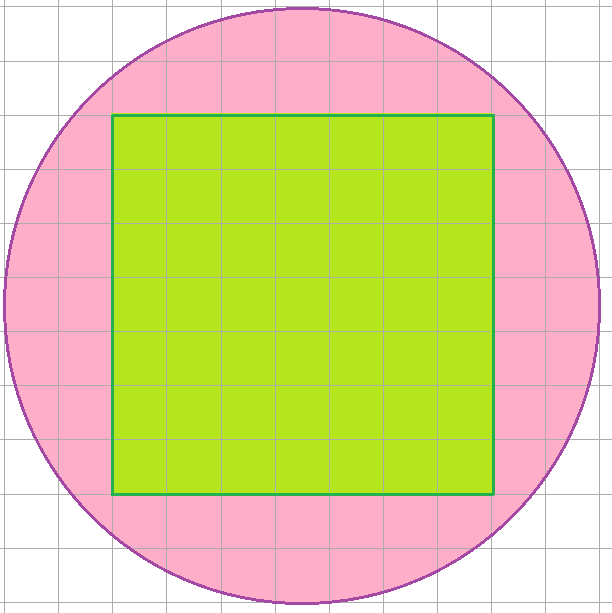
\includegraphics[width=0.45\linewidth]{../img/grid.png}}
			\caption{Розовым цветом отмечен $\Gamma_1$, салатовым -- $\underline{G} \textbackslash \Gamma_1$}  
		\end{minipage}
	\end{figure}
	
	\newpage
	
	\textbf{Задача 2.}\\
	Для уравнения переноса $\frac{\partial u}{\partial t} + a \frac{\partial u}{\partial x} = 0$ на равномерной сетке с шагами $\tau$ по $t$ и $h$ по $x$ найти условие спектральной устойчивости схемы Лакса:
	
	\begin{equation*}
		\frac{u_{k}^{n+1}-\frac{u_{k-1}^{n}+u_{k+1}^{n}}{2}}{\tau}+a \frac{u_{k+1}^{n}-u_{k-1}^{n}}{2 h}=0
	\end{equation*}
	
	Найти условие и порядок аппроксимирования этой схемой уравнения переноса.
	
	\textbf{Решение.}\\
	
	\begin{equation*}
		u_k^n = u(t_n, x_k)
	\end{equation*}
	
	Перепишем схему Лакса в другом виде:
	
	\begin{equation*}
		\frac{u_{k}^{n+1}-u_{k}^{n}}{\tau}+a \frac{u_{k+1}^{n}-u_{k-1}^{n}}{2 h}-\frac{u_{k+1}^{n}-2 u_{k}^{n}+u_{k-1}^{n}}{2 \tau}
	\end{equation*}
	
	Найдём условие и порядок аппроксимирования данной схемы:
	
	\begin{align*}
		&\frac{u(t+\tau, x)-u(t, x)}{\tau}=\frac{1}{\tau}\left(u(t, x)+\tau \frac{\partial u(t, x)}{\partial t}+\frac{\tau^{2}}{2} \frac{\partial^{2} u(t, x)}{\partial t^{2}}+\mathrm{O}\left(\tau^{3}\right)-u(t, x)\right)= \\
		&=\frac{\partial u(t, x)}{\partial t}+\frac{\tau}{2} \frac{\partial^{2} u(t, x)}{\partial t^{2}}+\mathrm{O}\left(\tau^{2}\right)
	\end{align*}
	
	Воспользуемся следствием исходного выражения:
	
	\begin{equation*}
		\frac{\partial^{2} u(t, x)}{\partial t^{2}}=a^{2} \frac{\partial^{2} u(t, x)}{\partial x^{2}}
	\end{equation*}
	
	Кроме того, известно, что:
	
	\begin{equation*}
		\frac{\partial u(t, x)}{\partial x}=\frac{u(t, x+h)-u(t, x-h)}{2 h}+\mathrm{O}\left(h^{2}\right) \textup{ -- центральная разностная производная}
	\end{equation*}
	
	и
	
	\begin{equation*}
		\frac{\partial^{2} u(t, x)}{\partial x^{2}}=\frac{u(t, x+h)-2 u(t, x)+u(t, x-h)}{h^{2}}+\mathrm{O}\left(h^{2}\right) \textup{ -- вторая разностная производная}
	\end{equation*}
	
	Тогда 
	
	\begin{equation*}
		\begin{array}{l}
			\frac{u_{k}^{n+1}-u_{k}^{n}}{\tau}+a \frac{u_{k+1}^{n}-u_{k-1}^{n}}{2 h}-\frac{a^{2} h^{2}}{2 \tau} \frac{u_{k+1}^{n}-2 u_{k}^{n}+u_{k-1}^{n}}{h^{2}}=\left.\frac{\partial u(t, x)}{\partial t}\right|_{t=t_{n}, x=x_{k}}+\left.\frac{\tau a^{2}}{2} \frac{\partial^{2} u(t, x)}{\partial x^{2}}\right|_{t=t_n, x=x_{k}}+O\left(\tau^{2}\right)+ \\
			+\left.a \frac{\partial u(t, x)}{\partial x}\right|_{t=t_{n}, x=x_{k}}+O\left(h^{2}\right)-\left.\frac{h^{2} a^{2}}{2 \tau} \frac{\partial^{2} u(t, x)}{\partial x^{2}}\right|_{t=t_{n}, x=x_{1}}+\tau O\left(h^{2}\right)
		\end{array}
	\end{equation*}
	
	
	Таким образом, схема будет аппроксимировать исходное уравнение при условии, что $h^2 = o(\tau)$ -- это и будет условием аппроксимирования. Тогда уравнение представимо в виде:
	
	\begin{equation*}
		\left.\frac{\partial u(t, x)}{\partial t}\right|_{t=t_{n}, x=x_{k}}+\left.a \frac{\partial u(t, x)}{\partial x}\right|_{t=t_{n}, x=x_{k}}+O\left(\tau^{2}+h^{2}\right)=0
	\end{equation*}
	
	
	То есть схема аппроксимирует исходное уравнением со вторым порядком аппроксимирования по времени и протяжённости.
	
	Согласно спектральному признаку, используем соотношения:
	
	\begin{equation*}
		u_{k}^{n}=e^{i \varphi k}, u_{k}^{n+1}=\lambda u_{k}^{n}=\lambda e^{i \varphi k}
	\end{equation*}
	
	
	Имеем:
	
	\begin{equation*}
		\frac{\lambda-\frac{e^{i \varphi}+e^{-i \varphi}}{2}}{\tau}+a \frac{e^{i \varphi}-e^{-i \varphi}}{2 h}=0
	\end{equation*}
	
	
	Тогда
	
	\begin{equation*}
		\lambda = \cos(\varphi) - i r \sin(\varphi),
	\end{equation*}
	
	где $r = \frac{a\tau}{h}$.
	
	Условие спектральной устойчивости $|\lambda| = \cos^2(\varphi) + r^2 \sin^2(\varphi) \leq 1$ выполняется при $r^2 \leq 1 \Leftrightarrow |r| \leq 1$.
	
	
	
\newpage

\textbf{Задача 3.}\\

Для уравнения переноса $\frac{\partial u}{\partial t} + a \frac{\partial u}{\partial x} = 0$ на равномерной сетке с шагами $\tau$ по $t$ и $h$ по $x$ найти условие спектральной устойчивости схемы Лакса-Вендроффа:

\begin{equation*}
\frac{u_{k}^{n+1}-u_{k}^{n}}{\tau}+a \frac{u_{k+1}^{n}-u_{k-1}^{n}}{2 h}=\frac{a^{2} \tau}{2} \frac{u_{k+1}^{n}-2 u_{k}^{n}+u_{k-1}^{n}}{h^{2}}
\end{equation*}

Найти условие и порядок аппроксимирования этой схемой уравнения переноса.

\textbf{Решение.}\\
	
Найдём порядок аппроксимирования:

\begin{align*}
	&\frac{u(t+\tau, x)-u(t, x)}{\tau}=\frac{1}{\tau}\left(u(t, x)+\tau \frac{\partial u(t, x)}{\partial t}+\frac{\tau^{2}}{2} \frac{\partial^{2} u(t, x)}{\partial t^{2}}+\mathrm{O}\left(\tau^{3}\right)-u(t, x)\right)=\\
	&=\frac{\partial u(t, x)}{\partial t}+\frac{\tau}{2} \frac{\partial^{2} u(t, x)}{\partial t^{2}}+\mathrm{O}\left(\tau^{2}\right).
\end{align*}
	
Используем следствие исходного выражения:

\begin{equation*}
	\frac{\partial^{2} u(t, x)}{\partial t^{2}}=a^{2} \frac{\partial^{2} u(t, x)}{\partial x^{2}}.
\end{equation*}	
	
Тогда

\begin{equation*}
	\frac{\partial u(t, x)}{\partial t}=\frac{u(t+\tau, x)-u(t, x)}{\tau}-\frac{a^{2} \tau}{2} \frac{\partial^{2} u(t, x)}{\partial x^{2}}+\mathrm{O}\left(\tau^{2}\right),
\end{equation*}
	
	Кроме того, известно, что:

\begin{equation*}
	\frac{\partial u(t, x)}{\partial x}=\frac{u(t, x+h)-u(t, x-h)}{2 h}+\mathrm{O}\left(h^{2}\right) \textup{ -- центральная разностная производная}
\end{equation*}

и

\begin{equation*}
	\frac{\partial^{2} u(t, x)}{\partial x^{2}}=\frac{u(t, x+h)-2 u(t, x)+u(t, x-h)}{h^{2}}+\mathrm{O}\left(h^{2}\right) \textup{ -- вторая разностная производная}
\end{equation*}
	
Используя обозначение $u_k^n = u(t_n,x_k)$, получим:

\begin{equation*}
	\begin{array}{l}
	\frac{u_{k}^{n+1}-u_{k}^{n}}{\tau}+a \frac{u_{k+1}^{n}-u_{k-1}^{n}}{2 h}-\frac{a^{2} \tau}{2} \frac{u_{k+1}^{n}-2 u_{k}^{n}+u_{k-1}^{n}}{h^{2}}=\left.\frac{\partial u(t, x)}{\partial t}\right|_{t=t_{n}, x=x_{k}}+\left.\frac{\tau a^{2}}{2} \frac{\partial^{2} u(t, x)}{\partial x^{2}}\right|_{t=t_n, x=x_{k}}+ \\
	+ O\left(\tau^{2}\right)+\left.a \frac{\partial u(t, x)}{\partial x}\right|_{t=t_{n}, x=x_{k}}+\mathrm{O}\left(h^{2}\right)-\left.\frac{\tau a^{2}}{2} \frac{\partial^{2} u(t, x)}{\partial x^{2}}\right|_{t=t_{n}, x=x_{k}}+\tau \mathrm{O}\left(h^{2}\right)=\\
	= \left.\frac{\partial u(t, x)}{\partial t}\right|_{t=t_{n}, x=x_{k}}+\left.a \frac{\partial u(t, x)}{\partial x}\right|_{t=t_n, x=x_{k}}+\mathrm{O}\left(\tau^{2}+h^{2}\right)
	\end{array}
\end{equation*}
	
Схема Лакса-Вендроффа аппроксимирует уравнение переноса со вторым порядком по $\tau$ и $h$.
	
Проверим условие спектральной устойчивости. Согласно спектральному признаку, используем соотношения:

\begin{equation*}
	u_{k}^{n}=e^{i \varphi k}, u_{k}^{n+1}=\lambda u_{k}^{n}=\lambda e^{i \varphi k}
\end{equation*}
	
Тогда имеем:

\begin{equation*}
	\frac{\lambda-1}{\tau}+a \frac{e^{i \varphi}-e^{-i \varphi}}{2 h}=\frac{a \tau^{2}}{h^{2}} \frac{e^{i \varphi}-2+e^{-i \varphi}}{h^{2}}
\end{equation*}

Отсюда:

\begin{equation*}
	\lambda=1-i r \sin \varphi-2 r^{2} \sin ^{2} \frac{\varphi}{2}
\end{equation*}

и

\begin{equation*}
	\begin{array}{l}
	|\lambda|=\left(1-2 r^{2} \sin ^{2} \frac{\varphi}{2}\right)^{2}+r^{2} \sin ^{2} \varphi=1-4 r^{2} \sin ^{2} \frac{\varphi}{2}+4 r^{4} \sin ^{4} \frac{\varphi}{2}+4 r^{2} \sin ^{2} \frac{\varphi}{2}\left(1-\sin ^{2} \frac{\varphi}{2}\right)= \\
	=1+4 r^{4} \sin ^{4} \frac{\varphi}{2}-4 r^{2} \sin ^{4} \frac{\varphi}{2} \leq 1
	\end{array}
\end{equation*}

То есть $|r| \leq 1$.






















	
	
\end{document}